\section{Frozen 2026 holdout results}
\label{sec:holdout}

\subsection{Evaluation population and point forecasting}

The frozen holdout covers 212 delivery days from 1 January through 31 July 2026. All 212 days satisfy the common economic-evaluation requirements. The point-forecast comparison contains 5,087 identical hourly observations.

\begin{table}[htbp]
\centering
\caption{Point-forecast performance in the frozen 2026 holdout.}
\label{tab:holdout_forecasts}
\begin{adjustbox}{max width=\textwidth}
\begin{tabular}{lrrrr}
\toprule
Model & MAE & RMSE & Median AE & \(N\) \\
\midrule
Lag-24 & 29.33 & 46.86 & 17.06 & 5,087 \\
Lag-168 & 36.01 & 56.60 & 22.94 & 5,087 \\
XGBoost Full & \textbf{17.51} & \textbf{29.87} & \textbf{11.99} & 5,087 \\
XGBoost Tier-1 & 24.36 & 38.41 & 15.77 & 5,087 \\
\bottomrule
\end{tabular}
\end{adjustbox}
\end{table}

\begin{figure}[htbp]
\centering
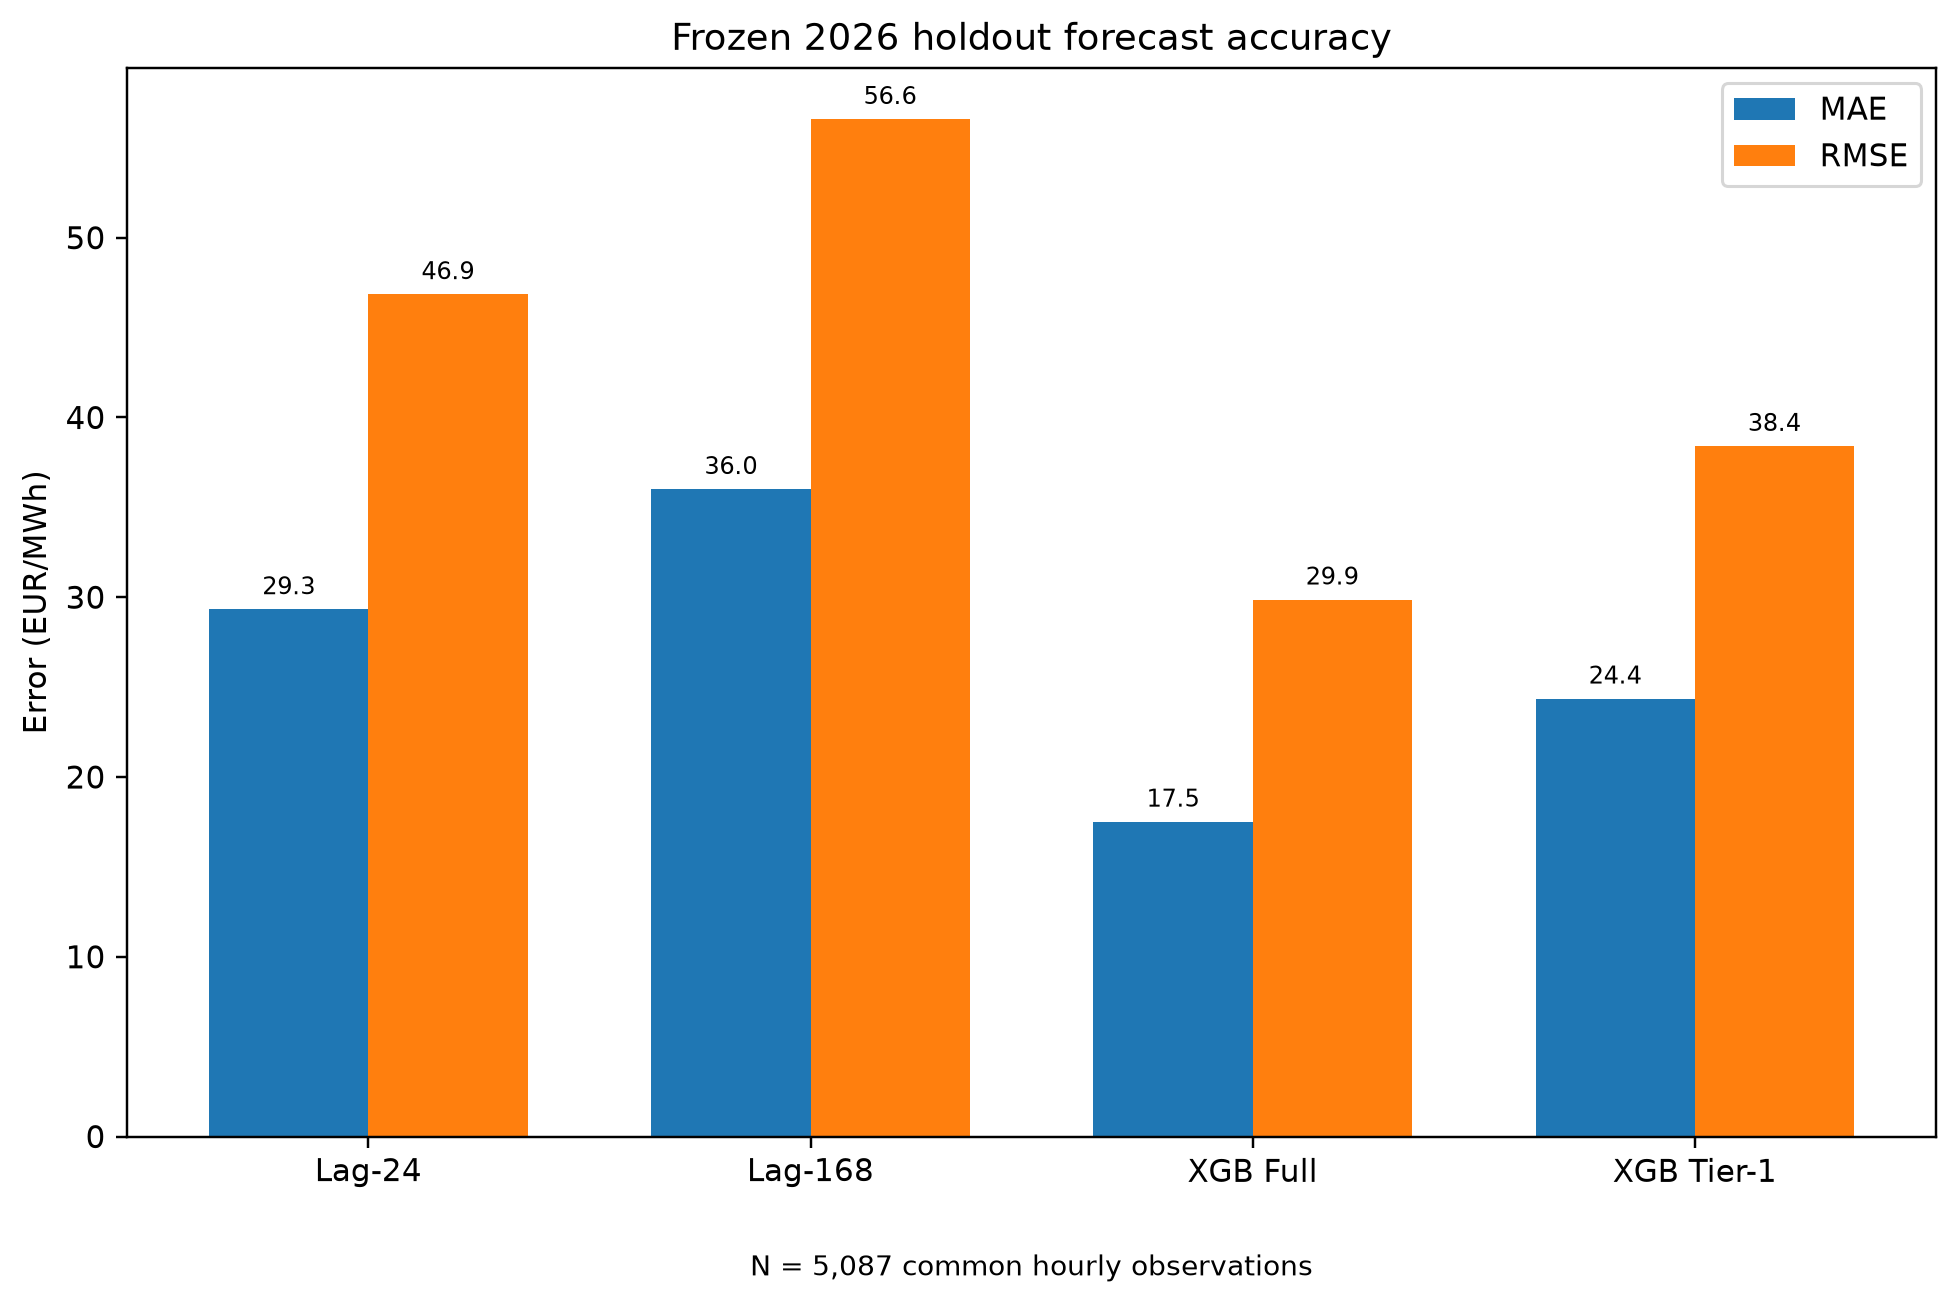
\includegraphics[width=0.92\linewidth]{figures/fig7_holdout_forecast_accuracy.png}
\caption{Point-forecast accuracy in the frozen 2026 holdout (\(N=5{,}087\) common hourly observations). Full XGBoost has the lowest MAE and RMSE, while Tier-1 XGBoost remains more accurate than both naive benchmarks.}
\label{fig:holdout_accuracy}
\end{figure}

Table~\ref{tab:holdout_forecasts} and Figure~\ref{fig:holdout_accuracy} show the same ranking. Full XGBoost reduces MAE by approximately 40.3\% relative to lag-24 and 51.4\% relative to lag-168. Tier-1 XGBoost also improves upon lag-24, with an MAE approximately 16.9\% lower, but remains materially weaker than Full.

\subsection{Primary economic results}

\begin{table}[htbp]
\centering
\caption{Frozen holdout strategy results at eta=0.85 and c=€10.}
\label{tab:holdout_strategy}
\begin{adjustbox}{max width=\textwidth}
\begin{tabular}{lrrrrr}
\toprule
Strategy & Trading days & Net P\&L & Profitable days & Hit rate & Worst day \\
\midrule
S0 & 0 & 0.00 & 0.0\% & -- & 0.00 \\
S1 & 208 & 18,564.42 & 84.0\% & 85.6\% & -67.28 \\
S2 & 210 & \textbf{20,002.02} & \textbf{91.0\%} & 91.9\% & -17.55 \\
S3 & 160 & 19,130.01 & 75.0\% & \textbf{99.4\%} & \textbf{-0.83} \\
S4 & 205 & 19,218.41 & 86.8\% & 89.8\% & -31.14 \\
S5 & 117 & 14,721.23 & 54.7\% & 99.1\% & -5.98 \\
\bottomrule
\end{tabular}
\end{adjustbox}
\end{table}

\begin{figure}[htbp]
\centering
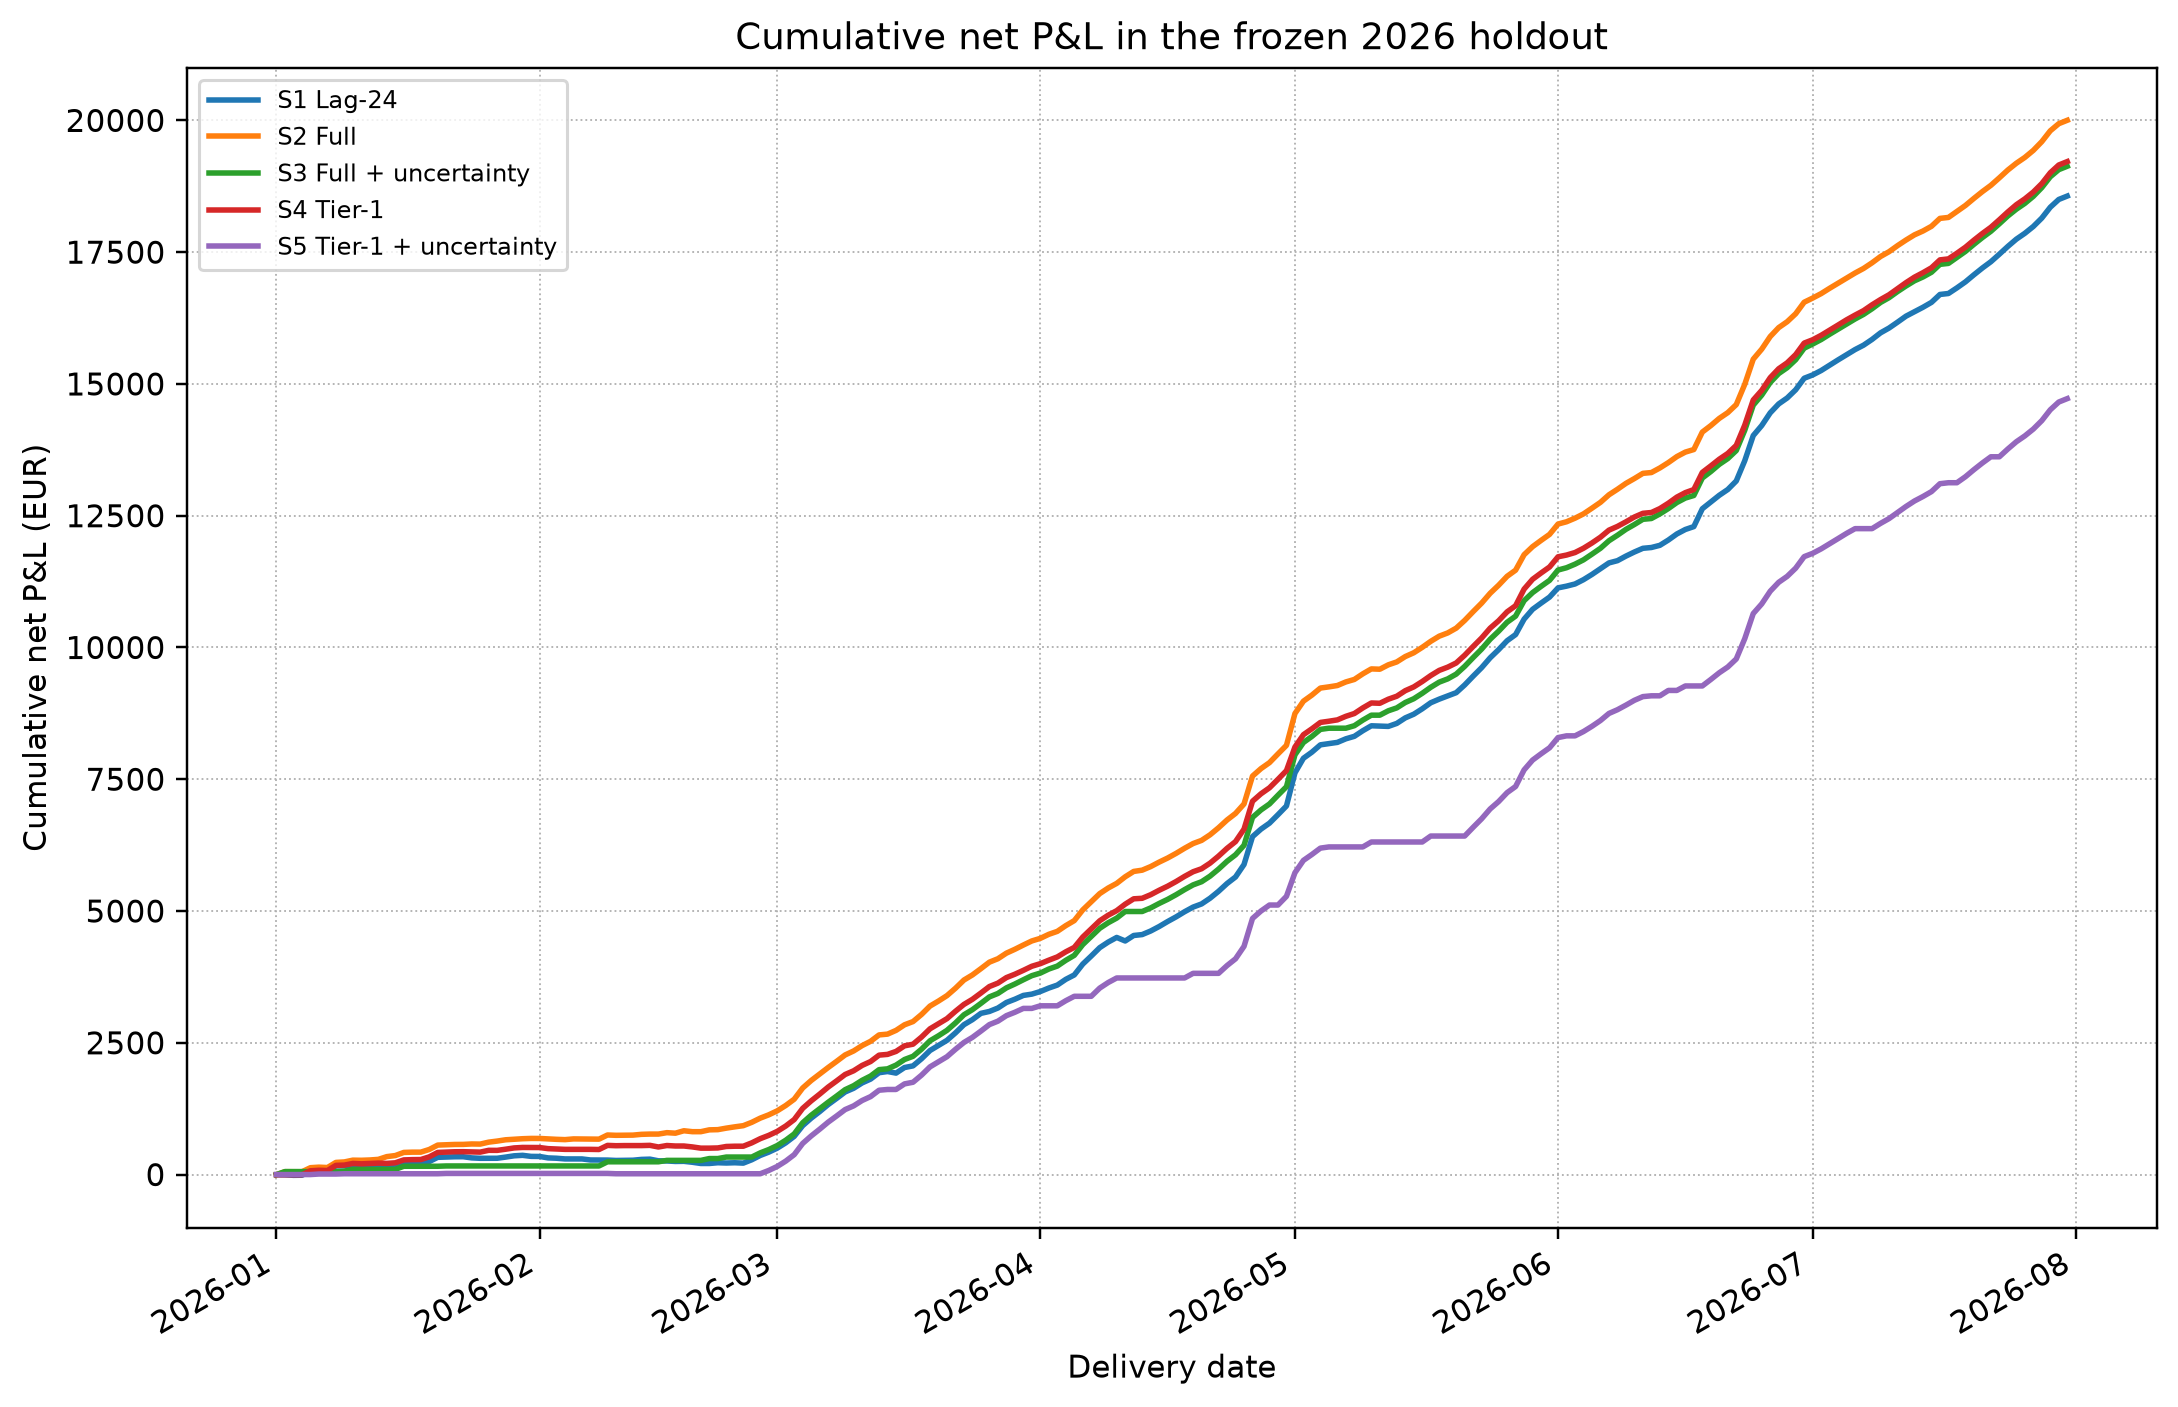
\includegraphics[width=\linewidth]{figures/fig8_holdout_cumulative_pnl.png}
\caption{Cumulative net P\&L over the 212-day frozen 2026 holdout. The curves are constructed directly from the preserved daily strategy results.}
\label{fig:cumulative_pnl}
\end{figure}

The primary contrast is
\[
\Delta_{forecast}=S2-S1=€1,437.60.
\]
Table~\ref{tab:holdout_strategy} summarizes the primary strategy outcomes, while Figure~\ref{fig:cumulative_pnl} shows their cumulative paths. The Full XGBoost point strategy earns approximately 7.7\% more cumulative net P\&L than the lag-24 strategy under the primary assumptions.

\subsection{Pre-specified nine-cell sign-consistency test}

\begin{table}[htbp]
\centering
\caption{Frozen holdout \(S2-S1\) sensitivity grid (EUR).}
\label{tab:holdout_grid}
\begin{adjustbox}{max width=\textwidth}
\begin{tabular}{rrrr}
\toprule
\(\eta_{rt}\) & \(c=5\) & \(c=10\) & \(c=15\) \\
\midrule
0.70 & 1,204.42 & 1,050.05 & 1,050.96 \\
0.85 & 1,386.14 & \textbf{1,437.60} & 1,364.73 \\
0.92 & 1,439.21 & 1,432.42 & 1,449.81 \\
\bottomrule
\end{tabular}
\end{adjustbox}
\end{table}

\begin{figure}[htbp]
\centering
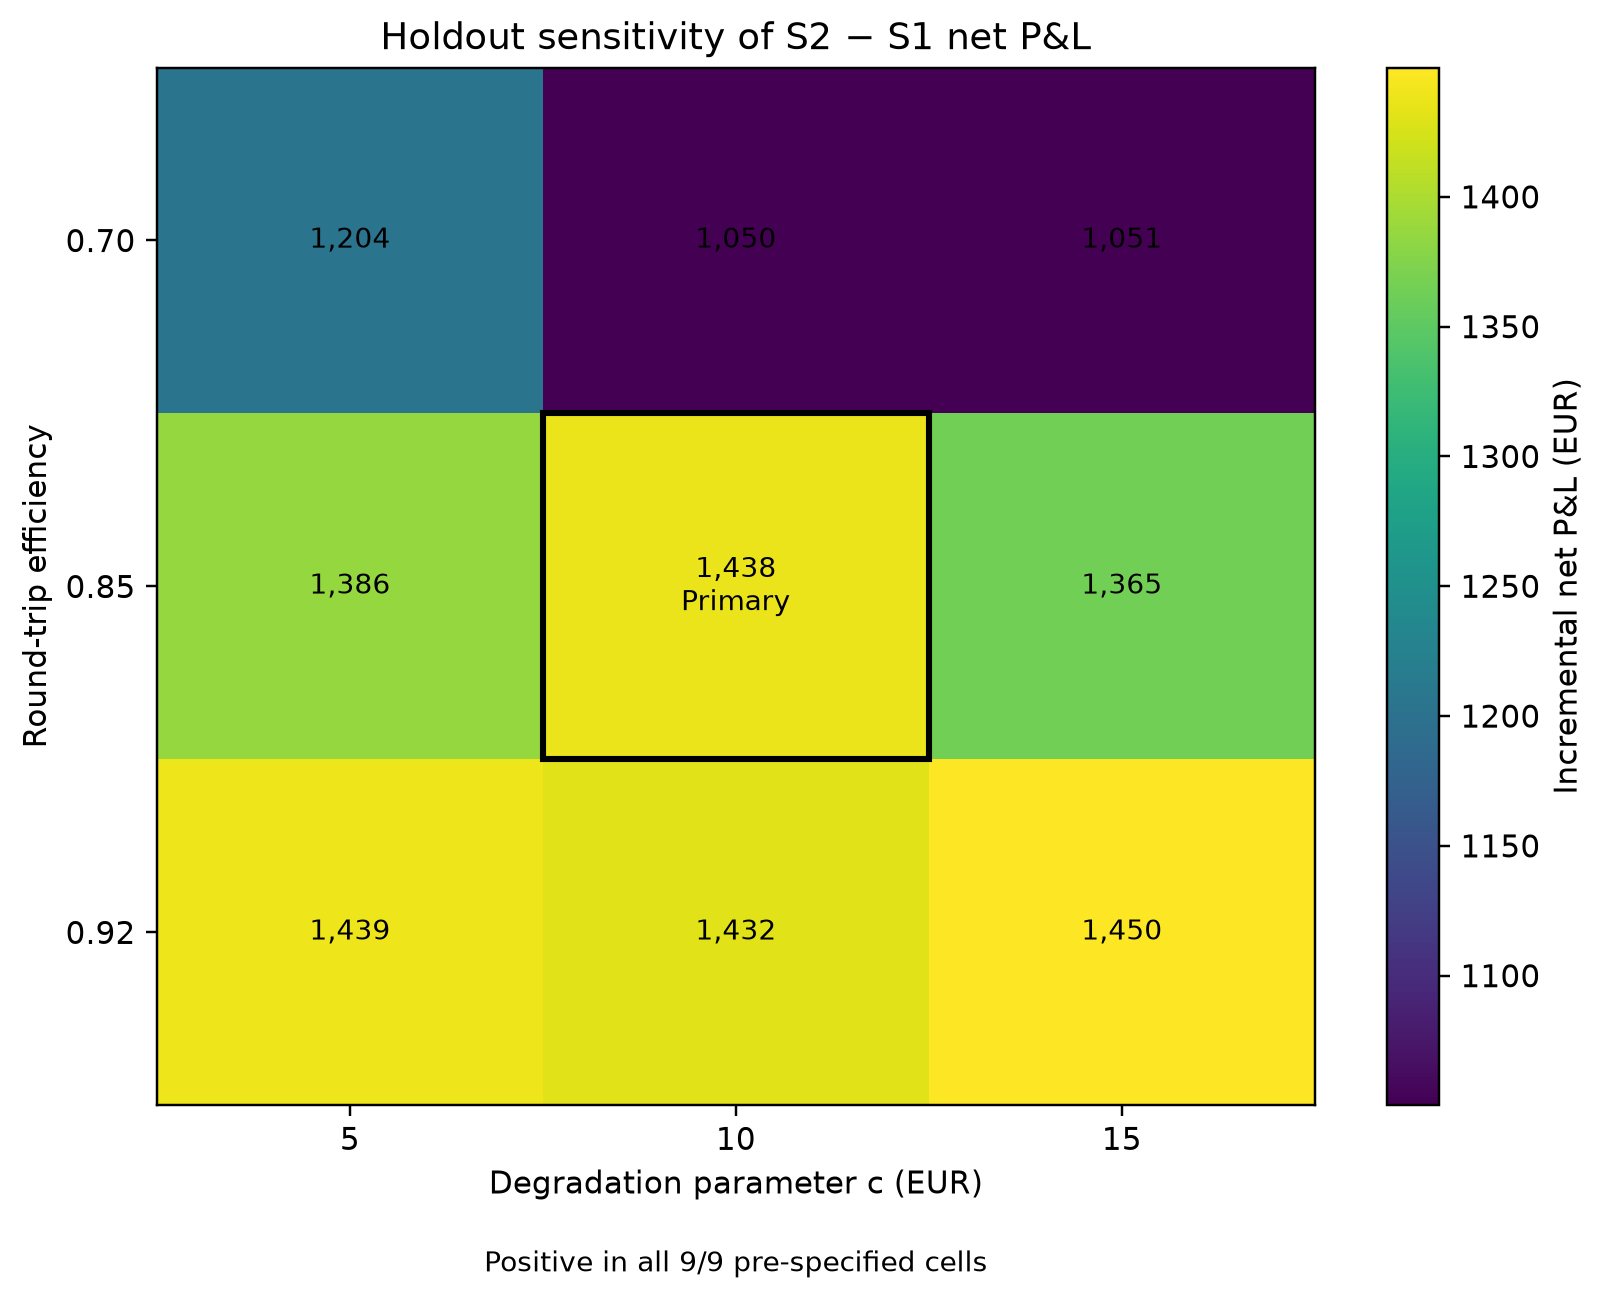
\includegraphics[width=0.88\linewidth]{figures/fig9_holdout_sensitivity_heatmap.png}
\caption{Sensitivity of the holdout forecast-value contrast \(S2-S1\) across the pre-specified efficiency and degradation-cost grid. Every cell is positive; the outlined cell is the primary setting.}
\label{fig:sensitivity_heatmap}
\end{figure}

Table~\ref{tab:holdout_grid} and Figure~\ref{fig:sensitivity_heatmap} show that the contrast is positive in all nine cells. Under the mechanical rule specified before holdout exposure, the primary forecast-value result therefore satisfies the pre-specified sign-consistency criterion. The nine cells are related sensitivity scenarios rather than independent statistical confirmations, and the criterion applies specifically to S2 over S1 under the frozen stylized contract.

\subsection{Uncertainty filtering}

The Full uncertainty-aware strategy earns €19,130.01 compared with €20,002.02 for S2, so
\[
\Delta_{uncertainty}=-€872.01.
\]

Consistent with the algebraic threshold identity in Section~\ref{sec:methods}, S2 and S3 both abstain on two days, S2 trades while S3 abstains on 50 days, and both trade on 160 days. Whenever both trade, the pair must be identical because the day-level threshold shifts every candidate pair score by the same amount; likewise, S3 cannot trade when S2 abstains. These are mechanical consequences of the frozen uncertainty construction rather than empirical discoveries.

The substantive empirical result is therefore the value of the additional abstention. The filter forgoes €952.46 of profitable opportunities and avoids €80.44 of losses, reconciling to the reported aggregate gap up to rounding.

The reduction in aggregate profit is accompanied by substantial downside improvement. The hit rate rises from 91.9\% to 99.4\%, the worst day improves from -€17.55 to -€0.83, and maximum drawdown improves from approximately -€22.61 to -€0.83.

\subsection{Tier-1 robustness}

At the primary parameters,
\[
S4=€19,218.41,
\]
giving
\[
\Delta_{Tier1}=S4-S2=-€783.61.
\]
The Tier-1 contrast is negative in all nine sensitivity cells.

The Tier-1 point estimate also exceeds lag-24:
\[
S4-S1=€653.99.
\]
This comparison was not one of the four pre-specified contrasts and is therefore reported descriptively rather than as a confirmatory economic result. In forecast accuracy, by contrast, Tier-1 materially improves on lag-24 while remaining weaker than Full.

Applying the uncertainty filter to Tier-1 produces S5, which trades on only 117 days with a 99.1\% hit rate and earns €14,721.23. It forgoes €4,654.82 of profitable outcomes while avoiding only €157.64 of losses relative to S4.

\subsection{Oracle value capture}

The ex-post oracle earns €21,243.10. The corresponding value-capture ratios are 87.4\% for S1, 94.2\% for S2, 90.1\% for S3, 90.5\% for S4 and 69.3\% for S5.

S2 therefore captures 94.2\% of the value available to the simplified perfect-hindsight oracle under the same one-cycle constraint. This ratio is a diagnostic property of the research contract, not an estimate of the fraction of real-world battery value captured.

\subsection{Tail-risk evidence}

\begin{table}[htbp]
\centering
\caption{Frozen holdout empirical daily-loss VaR and Expected Shortfall.}
\label{tab:holdout_tailrisk}
\begin{adjustbox}{max width=\textwidth}
\begin{tabular}{lrrrr}
\toprule
Strategy & VaR 95\% & ES 95\% & VaR 99\% & ES 99\% \\
\midrule
S1 & 9.72 & 26.16 & 29.64 & 48.31 \\
S2 & 2.07 & 7.07 & 8.35 & 13.45 \\
S3 & 0.00 & \textbf{0.08} & 0.00 & \textbf{0.39} \\
S4 & 5.09 & 13.02 & 20.60 & 26.82 \\
S5 & 0.00 & 0.56 & 0.00 & 2.82 \\
\bottomrule
\end{tabular}
\end{adjustbox}
\end{table}

Table~\ref{tab:holdout_tailrisk} shows that the holdout sample is too small for precise tail estimation. The 95\% tail contains only 10.6 effective observations and the 99\% tail 2.12. All holdout VaR and ES estimates are therefore flagged as low precision and used descriptively only.

\subsection{Stress-price days and concentration}

The holdout contains 69 negative-price days, 47 days with a price above €200/MWh and three days above €500/MWh. On negative-price days,
\[
\Delta_{forecast}=€153.01,
\]
while on the remaining days it is €1,284.58. On days above €200/MWh, the contrast remains positive at €262.60. The three days above €500/MWh yield identical cumulative P\&L across active strategies, so no separate inference is drawn from that very small subgroup.

S2's profits are not dominated by one extreme day: the top 1\%, 5\% and 10\% of holdout days account for 8.0\%, 18.6\% and 28.4\% of total S2 net P\&L, respectively.

\subsection{Post-hoc robustness analyses}
\label{sec:posthoc_results}

The following analyses were introduced only after exposure to the 2026 holdout and therefore do not alter the frozen primary result.

\paragraph{Stronger simple economic benchmarks.}
To compare XGBoost with simple rules that exploit recurring intraday structure, a weekday-aware naive benchmark and a trailing seven-day hourly mean profile were evaluated post hoc. The trailing-profile rule requires seven completed prior holdout days, so Table~\ref{tab:posthoc_benchmarks} uses the common 205-day sample from 8 January through 31 July 2026.

\begin{table}[htbp]
\centering
\caption{Post-hoc simple-benchmark comparison on the common 205-day sample.}
\label{tab:posthoc_benchmarks}
\begin{adjustbox}{max width=\textwidth}
\begin{tabular}{lrrrr}
\toprule
Strategy & MAE & RMSE & Net P\&L & Oracle share \\
\midrule
Lag-24 & 29.06 & 46.84 & 18,495.13 & 87.8\% \\
Weekday-aware naive & 29.89 & 47.77 & 18,372.81 & 87.2\% \\
Trailing 7-day mean profile & 29.28 & 43.59 & 19,630.98 & 93.2\% \\
XGBoost Tier-1 & 24.25 & 38.49 & 19,142.04 & 90.9\% \\
XGBoost Full & \textbf{17.51} & \textbf{30.06} & \textbf{19,869.02} & \textbf{94.3\%} \\
\bottomrule
\end{tabular}
\end{adjustbox}
\end{table}

Full XGBoost remains the most accurate model by a wide margin on this common sample, but the economic comparison is considerably tighter. Its net P\&L exceeds the trailing-profile rule by only €238.04. Tier-1 trails the trailing profile by €488.94. This shows that much of the economic value can be captured by a simple rule that learns the recurring hourly price shape, even though that rule has substantially worse point-forecast MAE than Full XGBoost.

\paragraph{Paired daily inference.}
Table~\ref{tab:posthoc_bootstrap} reports seven-day moving-block bootstrap intervals for selected daily P\&L contrasts. These intervals are supplementary and were not part of the frozen success criterion.

\begin{table}[htbp]
\centering
\caption{Post-hoc paired daily P\&L contrasts with 7-day moving-block bootstrap 95\% intervals.}
\label{tab:posthoc_bootstrap}
\begin{adjustbox}{max width=\textwidth}
\begin{tabular}{lrrrrr}
\toprule
Contrast & Days & Total difference & 95\% interval & Wins & Losses \\
\midrule
S2--S1 & 212 & 1,437.60 & [752.08, 2,140.98] & 95 & 63 \\
S3--S2 & 212 & -872.01 & [-1,459.21, -359.39] & 16 & 34 \\
S4--S2 & 212 & -783.61 & [-1,267.64, -348.12] & 49 & 97 \\
S5--S3 & 212 & -4,408.77 & [-6,189.90, -2,741.33] & 29 & 91 \\
S2--Trailing 7-day & 205 & 238.04 & [-110.21, 573.81] & 84 & 57 \\
\bottomrule
\end{tabular}
\end{adjustbox}
\end{table}

The frozen S2--S1 contrast remains positive under this supplementary paired analysis. By contrast, the Full XGBoost advantage over the post-hoc trailing-profile rule is much smaller and its block-bootstrap interval includes zero. The monthly S2--S1 decomposition is also uneven: January, February and March contribute €340.52, €367.45 and €300.87 respectively; April--June contribute €433.70 in total; July is approximately flat at -€4.94.

\paragraph{Holdout interval calibration.}
Table~\ref{tab:posthoc_calibration} summarizes post-hoc calibration of the nominal central 80\% intervals.

\begin{table}[htbp]
\centering
\caption{Post-hoc holdout calibration of the nominal central 80\% intervals.}
\label{tab:posthoc_calibration}
\begin{adjustbox}{max width=\textwidth}
\begin{tabular}{lrrrrr}
\toprule
Information set & Coverage & Lower miss & Upper miss & Mean width & Winkler score \\
\midrule
Full & 77.1\% & 9.7\% & 13.2\% & 45.12 & 89.25 \\
Tier-1 & 77.7\% & 11.3\% & 11.0\% & 71.72 & 135.31 \\
\bottomrule
\end{tabular}
\end{adjustbox}
\end{table}

Overall coverage is moderately below the nominal 80\% target for both information sets. Tier-1 achieves similar coverage only with intervals about 59\% wider than Full. Calibration is not stable over time: Full monthly coverage ranges from 69.7\% in March to 88.3\% in May, while Tier-1 ranges from 56.5\% in March to 92.2\% in May. Exploratory local-hour diagnostics also show lower Full coverage around several midday and evening hours, consistent with residual heteroskedasticity that is obscured by the pooled-hour residual construction.

\subsection{Holdout summary}

The first-look 2026 evidence supports the primary forecast-value result. Full XGBoost retains a large accuracy advantage, and the pre-specified economic contrast \(S2-S1\) is positive at the primary setting and in all nine sensitivity cells. Tier-1 has a higher economic point estimate than lag-24, but that non-pre-specified comparison is descriptive. The uncertainty-aware rule operates as an additional day-varying abstention threshold and trades aggregate profit for substantially greater selectivity and downside protection.
